\documentclass[main.tex]{subfiles}
\begin{document}
\newcommand\chapterlabel{gases}
\linenumbers


\chapter[Gases ]{Reactions in gase phase}

\begin{marginfigure}
      \begin{tikzpicture} \node (a) at (0,0) {\includegraphics[width=4cm]{chapter8/figure1}} node[rotate=90, font=\tiny] at ([yshift=.5cm,xshift=.1cm]a.south east) {\textsuperscript{\textcopyright} PngImg} ;
\end{tikzpicture}
\end{marginfigure}


\lettrine[lines=4]{\color{black!45}T}{he} air we all breath contains numerous gases, such as oxygen, nitrogen or carbon dioxide. Some of these gases are indeed essential for life. As an example, plants take up carbon dioxide to give off oxygen, and water is produced by the reaction of oxygen and hydrogen gas. Other gases are dangerous for life. An example is carbon monoxide, which results from gas stoves, heating systems and fire. This is a colorless, odorless, and tasteless gas that can bind to the blood displacing oxygen. As a consequence, carbon monoxide can build up in closed environments causing death. This chapter deals with the properties of gases. You will learn how to calculate the volume or pressure of a gas, characterizing its state. You will also learn how to work with mixtures of gases and for example predict the pressure of oxygen in an atmosphere containing numerous gases.




\begin{marginfigure}%LEARNING GOALS BOX
\begin{mytcbox}{GOALS}
\begin{enumerate}[label=\protect\circled{\color{white}\arabic*}]
\item Use the ideal and real gas law
\item Calculate partial pressures
\item Compute gas-property changes
\item Carry  stoichiometric calculations with volumes
\item Compute root square mean velocities
\end{enumerate}
\end{mytcbox}
\vspace{1cm}
\begin{tcolorbox}[enhanced,colback=red!5!white,colframe=black!50!red,boxrule=1pt,
  arc=0pt,outer arc=0pt,drop heavy lifted shadow]
\faGears\ 
\docenvdef{Discussion:} Explain why a hot air balloon rises up. Furthermore, why a He-filled birthday balloon rises while if you fill it with air it does no?
\end{tcolorbox}
\end{marginfigure}%LEARNING GOALS BOX


\section{Gases and its properties}
Gases contain atomic or molecular particles. They have very different properties than liquids or solids. The particles of a gas are spread and far away from each other. Liquids, on the other hand are made of loose particles that interact by means of weak forces. Solids on the other hand are packed materials and its particles, atoms or molecules, are closer together. This section covers the different properties of gases.

%\begin{tikzpicture}
%\flask{0,0}{0}{pomp};
%\flask[arrL]{5,0}{130}{ether};
%\flask[arrL]{10,0}{590}{ether};
%\end{tikzpicture}




\sloppy 
\begin{description}
\item[\docfilehook{Gases in the periodic table}{Gases in the periodic table}] 
Some of the elements in the periodic table are molecular gases, resulting of the combination of two atoms of the same element. For example, molecular oxygen (\ce{O2}) is gas. Similarly, molecular nitrogen (\ce{N2}), molecular hydrogen (\ce{H2}), molecular chlorine (\ce{Cl2}), or molecular fluorine (\ce{F2}) are all diatomic gases--they contain two atoms of the same element. Other gases result of the combination of two different non-metals. Examples are carbon monoxide (\ce{CO}) or dioxide (\ce{CO2}), and nitrogen monoxide (\ce{NO}) or dioxide (\ce{NO2}). The nobel gases (Ne, He, Ar) also exist in gas state.


\item[\docfilehook{Characteristics of gases}{Characteristics of gases}] 
Gases has different properties compared to solids of liquids:
\begin{itemize}
\item  Gases assume the volume and shape of its container. As they expand, they have no shape different than their container's shape.
\item Gases are compressible: they can be compressed, reducing its volume. Differently, liquids and solids are incompressible.
\item  The density of gases is small, compared to the one for solids and liquids.
\end{itemize}


%\begin{marginfigure}[0cm]%%%%%%%MARGIN FIGURE
%\includegraphics{chapter8/figure2}
%\caption{Oxygen is a flammable gas at room temperature.}
%\end{marginfigure}%%%%%%%MARGIN FIGURE
 
\item[\docfilehook{Volume, V}{Volume, V}] The volume of a gas (V) is the amount of space it occupies, and gases fully occupy the volume of its container. Liters (L) and milliliters (mL) are units of volume. Liter is a cubic unit and one litter equals to a cubic decimeter ($dm^3$). 
%\begin{equation*}
%\boxed{   \frac{1 \text{ L} }{1\text{ }dm^3}}\quad  \boxed{ \frac{1\text{ mL}}{1\text{ }cm^3}}   
%\end{equation*}
\item[\docfilehook{Temperature, T}{Temperature, T}] The temperature (T) of a gas is related to the speed (the average velocity) of its particles. The higher the temperature the higher the particles' speed. Although there are different units of temperature such as Kelvin (K) or celsius (C$^{\circ}$), in this chapter many formulas require the use of Kelvin temperature ($T_K$), that related to celsius ($T_C$) by the formula
\begin{equation*}
\boxed{   T_K=T_C+273}   
\end{equation*}
\item[\docfilehook{Amount of gas, n}{Amount of gas, n}] The amount of a gas (n) refers to the quantity of gas particles. The larger the amount of gas, the larger the amount of gas particles. The amount of gas is measured in moles or grams. Figure \ref{fig:{\chapterlabel}1} displays a list of all gas elements.
%\begin{marginfigure}[0cm]%%%%%%%MARGIN FIGURE
%\includegraphics{chapter8/figure4}
%\caption{Gas pressure is due to the collisions of the gas particles with the walls of its container.}
%\end{marginfigure}%%%%%%%MARGIN FIGURE

%%%%%%%%%%%%%%%%%%%%%%%%%%%%%
\begin{figure}[h] % FUL FIGURE
\begin{center}\GasTable\end{center}
\caption{Gas elements}
\label{fig:{\chapterlabel}1}
\end{figure}% FUL FIGURE
%%%%%%%%%%%%%%%%%%%%%%%%%%%%%










\item[\docfilehook{Pressure, P}{Pressure, P}] In general pressure is defined as force divided by surface. In the international system the unit of force is the Newton (N) and the unit of area (A) is the $\text{m}^2$. One newton is $1 \text{kg}\cdot \text{m}/\text{s}^2$.
\begin{equation*}
\boxed{   P=\frac{F}{A}
}   
\end{equation*}

   \begin{marginfigure}[2cm]
%   \begin{tikzpicture} \node (a) at (0,0) {\includegraphics[width=4cm, height=4cm]{chapter8/figure2}} node[rotate=90, font=\tiny] at ([yshift=.5cm,xshift=.1cm]a.south east) {\textsuperscript{\textcopyright} www.wallpaperflare.com} ;
%\node[text width=5cm] at ([yshift=0.2cm]a.north) {\mytriangle{red}Oxygen oxidizing is a gas};
%\end{tikzpicture}
\begin{tikzpicture} \node (a) at (0,0) {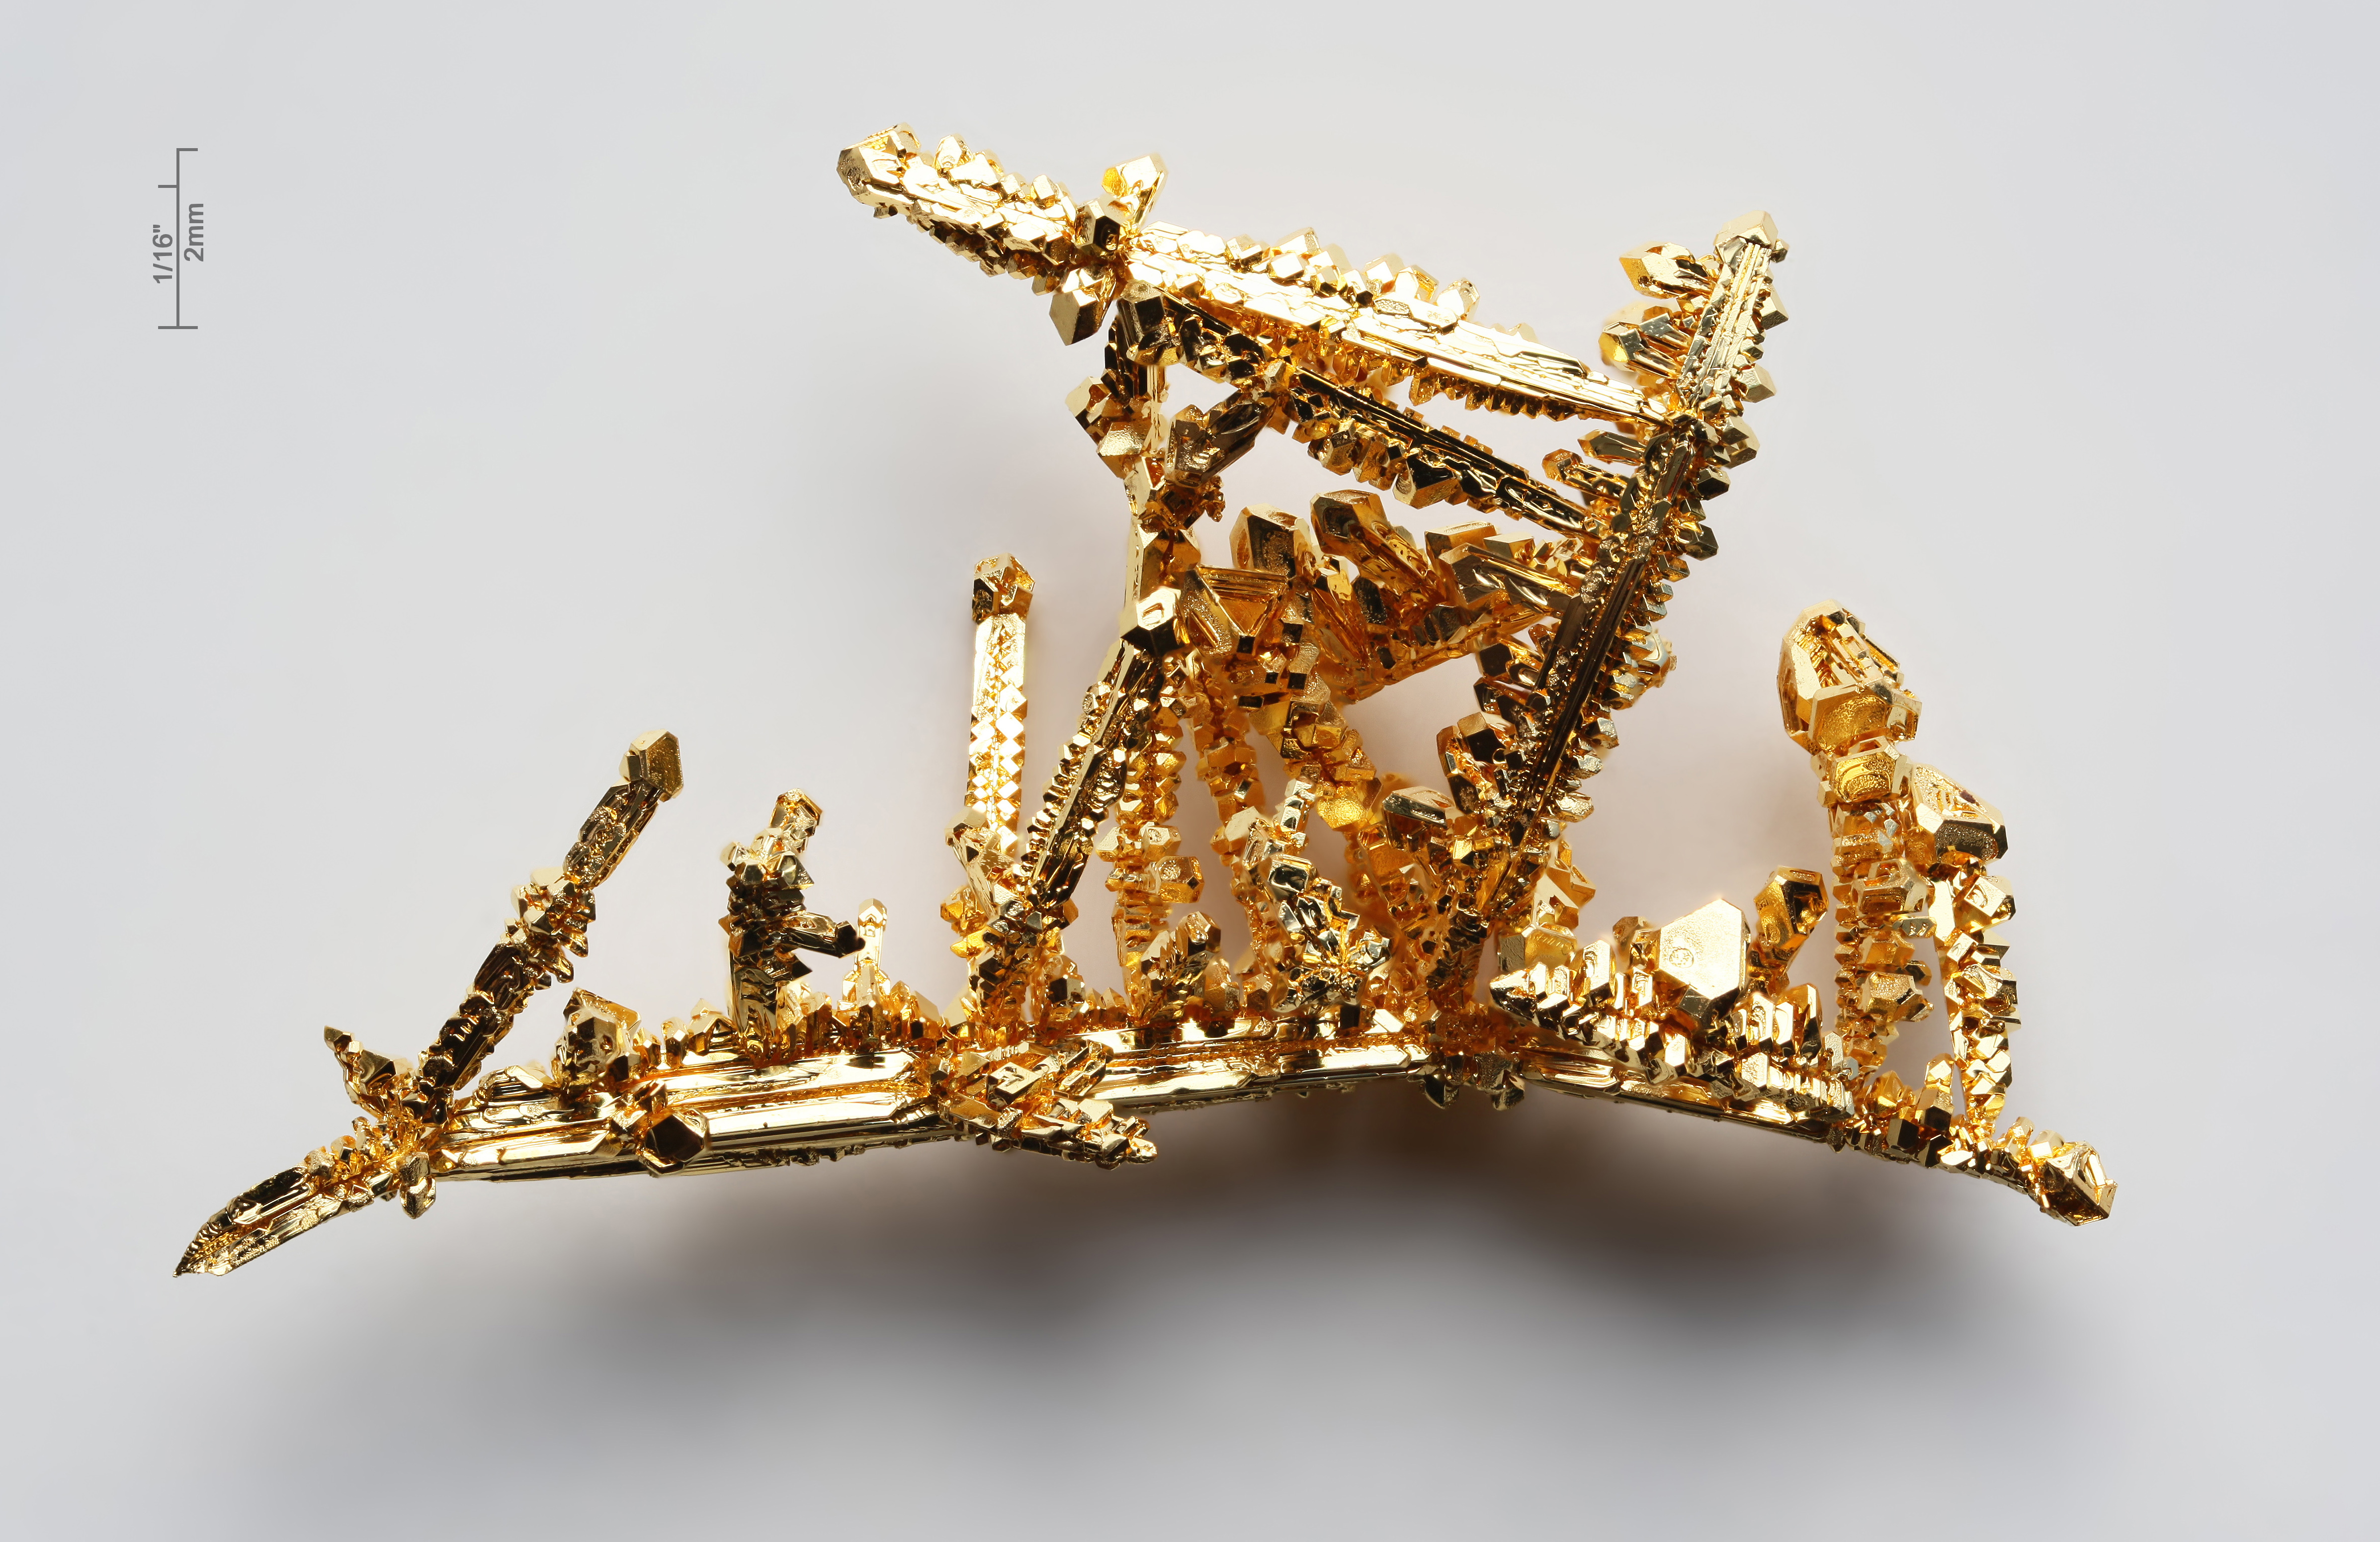
\includegraphics[width=4.5cm, height=4.5cm]{chapter8/figure6}} node[rotate=90, font=\tiny] at ([yshift=.5cm,xshift=.1cm]a.south east) {\textsuperscript{\textcopyright} www.wallpaperflare.com} ;
\node[text width=5cm] at ([yshift=0.2cm]a.north) {\mytriangle{red}Chlorine reactive is a gas};
\end{tikzpicture}
\begin{tikzpicture} \node (a) at (0,0) {\includegraphics[width=5cm, height=3cm]{chapter8/figure7}} node[rotate=90, font=\tiny] at ([yshift=.5cm,xshift=.1cm]a.south east) {\textsuperscript{\textcopyright} wikipedia} ;
\node[text width=5cm] at ([yshift=0.2cm]a.north) {\mytriangle{red}Hydrogen is a flammable gas used to power some cars};
\end{tikzpicture}
\caption{Examples of gases}
\label{fig:{\chapterlabel}4}
\end{marginfigure}




The particles of a gas are constantly moving. On its movement, they frequently hit the walls of its container, like the raindrops hitting the ceiling when it rains. When they hit the walls they exert a pressure, and pressure is defined as the force acting on certain area. The larger pressure the stronger the collisions with the walls and the higher the frequency of collision--the stronger the force applied on the walls. Imagine you are driving a motorcycle. While you drive you can feel the collision of the air's particle with your face. The faster you go the higher pressure. 
The value of air's pressure is measured with a barometer and depends on your location on the earth--in particular your altitude--as well as the weather. If you are at the sea level the atmospheric pressure is one unit of pressure (one atm), due to the air that you have on top of you. If you climb a mountain, the pressure decreases, as there is less air on top of you. The higher you are with respect to the sea level, the lower the air pressure. The weather also affects pressure, and in hot days the pressure of air is higher, whereas on a cold day pressure is lower. \\
Units of pressure are: bars, atmospheres (atm), torr, pascals (Pa) or millimeters of mercury (mmHg). In order to covert pressure units, you can use the following conversion factors:%\resizeableyellownote{2.5}{1}{Add these conversions into your flashcard.}
\begin{equation*}
\boxed{   \frac{1 \text{ atm} }{1.01325\text{ bar} }}\quad    \boxed{ \frac{1 \text{ atm} }{760\text{ mmHg} }}\quad  \boxed{ \frac{1\text{ torr}}{1\text{ mmHg}}}\quad  \boxed{ \frac{1\text{ atm}}{101325\text{ Pa}}}   
\end{equation*}
one millimeters of mercury (mmHg) is the same as 1 torr. As a note, the name torr knowledges the person who invented the barometer: Torricelli, an Italian physicist.


\begin{example} %%%%%%%%%%%%%%%%%%%%%%%% EXAMPLE BOX
An oxygen sample has a pressure of 2 atm. Convert this value to: (a) mmHg and (b) Pascals.
\\
\textlcsc{ \textcolor{dgreen}{\Large \textbf{Solution}} }\\
(a) we start by placing the given data (2 atm) and using the conversion factor between atm and mmHg, with the atm unit on the bottom, so that the units cancel
\begin{equation*}
2   \cancel{\text{ atm }} \times
\dfrac{760\text{ mmHg}  } {1\cancel{\text{ atm}}}=1520\text{mmHg}
\end{equation*}
(b) we proceed as in (a) but using the conversion between atm and Pa:
\begin{equation*}
2   \cancel{\text{ atm }} \times
\dfrac{101325\text{ Pa}  } {1\cancel{\text{ atm}}}=2.02\times 10^{5}\text{Pa}
\end{equation*}
\\
\faDiamond\ \textlcsc{ \textcolor{dgreen}{\Large \textbf{Study Check}} }\\
An oxygen sample has a pressure of 730 mmHg. Convert this value to atmospheres.
\\
\flushright Answer: 0.96 atm.
\end{example}%%%%%%%%%%%%%%%%%%%%%%%% EXAMPLE BOX


\item[\docfilehook{Measuring pressure}{Measuring pressure}] 
Two different devices are used to measure pressure, barometers and manometers. Barometer are used to measure specifically the atmospheric pressure and historically, they consist on a glass tube filled with mercury (\ce{Hg}), inverted on a plate containing more mercury. At the sea level, the height of the mercury columns should be close to 760mmHg.
Manometers, on the other hand, are used to measure the pressure of any gas. Manometers, like the one shown in Figure \ref{fig:{\chapterlabel}2}, consist of a u-shaped tube filled with mercury. There are two types of manometers: open-tube and closed-tube manometers.


%%%%%%%%%%%%%%%%%%%%%%%%%%%%%%%%
\begin{figure}%%%%%%%%%%%%%%%%%%%%%%%%%
\begin{tikzpicture}
\tikzset{edge/.style = {->,> = latex'}}
\def\r{1.1}% Mid-tube radius
\def\t{.2} % Tube thickness
\def\h{5}  % Straight height (total height is \r + \t/2 + \h)
\def\lh{2} % Left height
\def\rh{4} % Right height
\path [pattern=north west lines, pattern color=green]
  (-\r+\t/2, \lh) -- ++(0, -\lh) arc (180:360:\r-\t/2) |-
  ( \r+\t/2, \rh) -- ++(0, -\rh) arc (360:180:\r+\t/2) |- cycle;
\draw (-\r-\t/2, \lh-0.02) -- ++(\t,0)	 (\r-\t/2, \rh) -- ++(\t,0); 
%\draw [black, thick] 
%  (-\r-\t/2, \h) -- ++(0, -\h) arc (180:360:\r+\t/2) -- ++(0, \h)
%  (-\r+\t/2, \h) -- ++(0, -\h) arc (180:360:\r-\t/2) -- ++(0, \h);
\draw [black, thick] 
  (-\r-\t/2, \h) -- ++        (0, -\h) arc (180:360:\r+\t/2) -- ++(0, \h)
  (-\r+\t/2, \h) -- ++    (0, -\h) arc (180:360:\r-\t/2) -- ++(0, \h);
\draw [white, thick, fill=red!10] 
(-\r-\t/2+.1, \h     -1) -- ++ (-\r-2*\t/2, \h-0.1*\h-0.14cm) arc (0:350:1.0) -- ++ (\r+2*\t/2, \h-0.1*\h-0.16cm) |- cycle ;

 \draw[red!10,  fill=red!10]  (-\r-\t/2, 2.5*\lh) -- ++(\t-0.02,0) -- ++(0, -1.5*\lh) -- ++(-\t+0.04,0)  |- cycle ;
  \draw[black, thick]  (-\r-\t/2, 2.5*\lh-0.01) -- ++(\t,0)  ;
  \draw[black, thick]  (\r-\t/2, \rh+1.0) -- ++(\t,0)  ;  % Open close
\node [shift={(1.2,5.2)}, font=\small,scale=0.7] {Closed};% Open close

\node [shift={(-3.5,4.1)}] {Gas};

\draw[<->] (-0,2) -- (-0,4) ;
\draw[dash pattern=on \pgflinewidth off 2pt] (-0,2) -- (-.9,2)   (-0,4) -- (.9,4);

\node [shift={(0.2,3.1)}] {\small $\Delta$h};
\node [shift={(0.2,-1.8)}] {\small $\text{P}^{closed}=\Delta \text{h}\text{dg}$};
\draw[thin] (-1,0) -- ++(-.6,0) node [left,fill=white,font=\small,scale=0.7] {mercury};
\draw[thin] (1,4.5) -- ++(-.3,0) node [left,fill=white,font=\small,scale=0.7] {vacuum};

\begin{scope}[xshift = 6cm]
\path [pattern=north west lines, pattern color=green]
  (-\r+\t/2, \lh) -- ++(0, -\lh) arc (180:360:\r-\t/2) |-
  ( \r+\t/2, \rh) -- ++(0, -\rh) arc (360:180:\r+\t/2) |- cycle;
\draw (-\r-\t/2, \lh-0.02) -- ++(\t,0)	 (\r-\t/2, \rh) -- ++(\t,0); 
%\draw [black, thick] 
%  (-\r-\t/2, \h) -- ++(0, -\h) arc (180:360:\r+\t/2) -- ++(0, \h)
%  (-\r+\t/2, \h) -- ++(0, -\h) arc (180:360:\r-\t/2) -- ++(0, \h);
\draw [black, thick] 
  (-\r-\t/2, \h) -- ++        (0, -\h) arc (180:360:\r+\t/2) -- ++(0, \h)
  (-\r+\t/2, \h) -- ++    (0, -\h) arc (180:360:\r-\t/2) -- ++(0, \h);
\draw [white, thick, fill=red!10] 
(-\r-\t/2+.1, \h     -1) -- ++ (-\r-2*\t/2, \h-0.1*\h-0.14cm) arc (0:350:1.0) -- ++ (\r+2*\t/2, \h-0.1*\h-0.16cm) |- cycle ;

 \draw[red!10,  fill=red!10]  (-\r-\t/2, 2.5*\lh) -- ++(\t-0.02,0) -- ++(0, -1.5*\lh) -- ++(-\t+0.04,0)  |- cycle ;
  \draw[black, thick]  (-\r-\t/2, 2.5*\lh-0.01) -- ++(\t,0)  ;
 % \draw[black, thick]  (\r-\t/2, \rh+1.0) -- ++(\t,0)  ;  % Open close
\node [shift={(1.2,5.2)}, font=\small,scale=0.7] {Open};% Open close

\node [shift={(-3.5,4.1)}] {Gas};

\draw[<->] (-0,2) -- (-0,4) ;
\draw[dash pattern=on \pgflinewidth off 2pt] (-0,2) -- (-.9,2)   (-0,4) -- (.9,4);

\node [shift={(0.2,3.1)}] {\small $\Delta$h};
\node [shift={(0.2,-1.8)}] {\small $\text{P}^{open}=\Delta \text{h}\text{dg}+\text{P}_{atm}$};
\draw[thin] (1,4.5) -- ++(-.3,0) node [left,fill=white,font=\small,scale=0.7] {atmosphere};

\end{scope}
\end{tikzpicture}
\caption{Two types of manometers: open-tube and closed-tube manometer}
\label{fig:{\chapterlabel}2}
\end{figure}%%%%%%%%%%%%%%%%%%%%%%%%%%%
%%%%%%%%%%%%%%%%%%%%%%%%%%%%%%%%




The pressure exerted by a gas changes level of mercury on both sides of the tube and the difference in height measured as the right minus the left side ($\Delta h=h_{right}-h_{left}$) is related to the gas pressure. For closed-tube manometers--normally used to measure pressured below the atmospheric pressure--when the gas pressure increases the left column of the barometer is reduced and the right column increases. The difference between both columns is related to the gas pressure by means of:
\begin{equation}
\boxed{   \text{P}^{closed}=\text{hdg}} \quad\quad\quad  \boxed{ \text{P}^{open}=\text{hdg}+\text{P}_{atm}}    
\end{equation}
where:
\begin{where}
 \item P   is the pressure of the gas in Pa
\item $\Delta$h is the heigh difference in m, measured as $h_{right}-h_{left}$
 \item d   is the density of mercury 13593 kg/$\text{m}^3$
\item g   is gravity, 9.8 m/$\text{s}^2$
\item $\text{P}_{atm}$   is the atmospheric pressure close to 101325 Pa
\end{where}

For the open-tube manometer, normally used to measure pressured above the atmospheric pressure, we need to take into account the atmospheric pressure to the gas pressure. For this type of manometers, if the left column is below the right column ($\Delta h=h_{right}-h_{left}<0$), this means that the pressure of in the gas is below the atmospheric pressure.




\end{description}



%%%%%%%%%%%%%%%%%%%%%%%%%%%%%%%%%%
\begin{figure*}
\resizebox{.9\textwidth}{!}{
	  \begin{tikzpicture} \node (a) at (0,0) {\includegraphics[width=4.5cm, height=4.5cm]{chapter8/figure3}} node[rotate=90, font=\tiny] at ([yshift=.5cm,xshift=.1cm]a.south east) {\textsuperscript{\textcopyright} wikipedia} ;
\node[text width=5cm] at ([yshift=0.8cm]a.north) {\baselineskip=8pt \mytriangle{red}{\small A barometer used to measure the atmospheric pressure}};
 
 \node (b) at (6cm,0) {\includegraphics[width=4.5cm, height=4.5cm]{chapter8/figure4}} node[rotate=90, font=\tiny] at ([yshift=.5cm,xshift=.1cm]b.south east) {\textsuperscript{\textcopyright} wikipedia} ;
\node[text width=4cm] at ([yshift=0.8cm]b.north) {\mytriangle{red}{\small A manometer used to measure gas pressures}};

 \node (c) at (12cm,0) {\includegraphics[width=5cm, height=5cm]{chapter8/figure5}} node[rotate=90, font=\tiny] at ([yshift=.5cm,xshift=.1cm]c.south east) {\textsuperscript{\textcopyright} PxFuel} ;
\node[text width=4cm] at ([yshift=0.8cm]c.north) {\mytriangle{red}{\small A pressure gauge}};
\end{tikzpicture}
}

\caption{Pressure measuring devices}
\label{fig:{\chapterlabel}3}
\end{figure*}
%%%%%%%%%%%%%%%%%%%%%%%%%%%%%%%%%%






\section{Ideal gas law}
Ideal gases are gases made of particles without a size (very tinny) that do not interact with each other. The temperature, pressure, volume and number of moles of a gas are not independent. They are related by the ideal gas law. In this section we will introduce this law in two different forms: in terms of volume and in terms of density.
\sloppy 
\begin{description}
\item[\docfilehook{Ideal gas law in terms of moles}{Ideal gas law in terms of moles}] 
The ideal gas law says:%\resizeableyellownote{2.5}{1}{Add this formula to your flashcard.}

\begin{equation*}\begin{split}
\boxed{  PV=nRT} \quad \textcolor{blue}{\text{Ideal Gas Law}}
\end{split}\end{equation*}
where:
\begin{where}
 \item $P$   is the pressure of the gas in atm
\item $V$    is the volume of the gas in L 
 \item $n$   is the number of moles of the gas
\item $T$   is the temperature of the gas in K
\item $R$   is the constant of the gas $0.082\frac{\text{atm}\cdot \text{L}}{\text{mol}\cdot \text{K}}$
\end{where}
Imagine for example that you inflate a balloon with you mouth, introducing air particles into the balloon.
While the number of particles inside the balloon grows, its volume will grow too. More particles will collide with the walls of the balloon and hence, the pressure inside the balloon will also increase. 

\begin{example} %%%%%%%%%%%%%%%%%%%%%%%% EXAMPLE BOX
Helium gas is used to inflate blimps, scientific balloons and party balloons. What is the volume in litters of a 0.2 moles of Helium balloon at 300K and 2 atm.
\\
\textlcsc{ \textcolor{dgreen}{\Large \textbf{Solution}} }\\
%%% DATA BOX
\begin{tcbitemize}[raster columns=3, raster rows=3, enhanced, sharp corners, raster equal height=rows, raster force size=false, raster column skip=0pt, raster row skip = 0pt]
%Empty corner and two headers
\tcbitem[blankest, width=1cm]
\tcbitem[header = helpful]
\texta
\tcbitem[header = harmful]
\textb
%First row
\tcbitem[firstcol = internal]
\textcn
\tcbitem[swotbox = G]
$T=300K$\\
$P=2atm$\\
$n=0.2mol$\\
$R=0.082\frac{\text{atm}\cdot \text{L}}{\text{mol}\cdot \text{K}}$\\
\tcbitem[swotbox = A]
$V$\\
\\
\\
\\
\end{tcbitemize}%%% DATA BOX
Using now the ideal gases formula: $PV=nRT$, we have
\begin{equation*}
2 \cancel{\text{atm}}\cdot V=0.2\cancel{\text{mol}}\cdot 0.082\frac{\cancel{\text{atm}}\cdot \text{L}}{\text{mol}\cdot \cancel{\text{K}}}\cdot 300\cancel{K}
\end{equation*}
All units but L cancel out. Solving for V we have 2.46 L.
\\
\faDiamond\ \textlcsc{ \textcolor{dgreen}{\Large \textbf{Study Check}} }\\
What is the pressure in atmospheres of a 1 L balloon containing 3 moles of Helium at 40C$^{\circ}$.
\\
\flushright Answer: 77.00 atm.
\end{example}%%%%%%%%%%%%%%%%%%%%%%%% EXAMPLE BOX

\item[\docfilehook{Ideal gas law in terms of density}{Ideal gas law in terms of density}] 
The ideal gas law in terms of density is:%\resizeableyellownote{2.5}{1}{Add this formula to your flashcard.}

\begin{equation*}\begin{split}
\boxed{  P\cdot MW=DRT} \quad \textcolor{blue}{\text{Ideal Gas Law in terms of D}}
\end{split}\end{equation*}
where:
\begin{where}
 \item $P$   is the pressure of the gas in atm
\item $MW$ is the molecular weight (or atomic weight, AW) of the gas in g/mol 
 \item $D$   is the density in $g\cdot L^{-1}$
\item $T$   is the temperature of the gas in K
\item $R$   is the constant of the gas $0.082\frac{\text{atm}\cdot \text{L}}{\text{mol}\cdot \text{K}}$
\end{where}
We use this formula when we are questioned about the molar mass or density of the gas.

\begin{example} %%%%%%%%%%%%%%%%%%%%%%%% EXAMPLE BOX
What is the density of Helium balloon at 400K and 3 atm.
\\
\textlcsc{ \textcolor{dgreen}{\Large \textbf{Solution}} }\\
Besides the data in the problem, as the gas is He we already know its atomic mass from the periodic table:
%%% DATA BOX
\begin{tcbitemize}[raster columns=3, raster rows=3, enhanced, sharp corners, raster equal height=rows, raster force size=false, raster column skip=0pt, raster row skip = 0pt]
%Empty corner and two headers
\tcbitem[blankest, width=1cm]
\tcbitem[header = helpful]
\texta
\tcbitem[header = harmful]
\textb
%First row
\tcbitem[firstcol = internal]
\textcn
\tcbitem[swotbox = G]
$T=400K$\\
$P=3atm$\\
$AW=4 g\cdot mol^{-1}$\\
$R=0.082\frac{\text{atm}\cdot \text{L}}{\text{mol}\cdot \text{K}}$\\
\tcbitem[swotbox = A]
$D$\\
\\
\\
\\
\end{tcbitemize}%%% DATA BOX
Using now the ideal gases formula in terms of density: $P\cdot MW=DRT$, we have
\begin{equation*}
3 \cancel{\text{atm}}\cdot 4\frac{g}{\cancel{\text{mol}}}=D\cdot 0.082\frac{\cancel{\text{atm}}\cdot \text{L}}{\cancel{\text{mol}}\cdot \cancel{\text{K}}}\cdot 400\cancel{K}
\end{equation*}
Solving for D we have 0.36 $g\cdot L^{-1}$.
\\
\faDiamond\ \textlcsc{ \textcolor{dgreen}{\Large \textbf{Study Check}} }\\
What is the molecular mass of a 4 $g\cdot L^{-1}$ density gas at 30C$^{\circ}$ and 5 atm.
\\
\flushright Answer: 19.87 g/mol.
\end{example}%%%%%%%%%%%%%%%%%%%%%%%% EXAMPLE BOX
\item[\docfilehook{STP conditions}{STP conditions}] 
STP conditions refer to standard temperature (273K) and pressure (1 atm) conditions. Working at STP conditions means pressure will be fixed at 1 atm and temperature at 273K.%\resizeableyellownote{2.5}{1}{Add this relation into your flashcard.}
\begin{equation*}
\boxed{  \text{1 atm and 273K}  } \quad \textcolor{blue}{\text{STP Conditions}}
\end{equation*}
\begin{example} %%%%%%%%%%%%%%%%%%%%%%%% EXAMPLE BOX
Calculate the volume in litters of 5 moles of nitrogen at STP conditions.
\\
\textlcsc{ \textcolor{dgreen}{\Large \textbf{Solution}} }\\
From the problem we have the following data:
%%% DATA BOX
\begin{tcbitemize}[raster columns=3, raster rows=3, enhanced, sharp corners, raster equal height=rows, raster force size=false, raster column skip=0pt, raster row skip = 0pt]
%Empty corner and two headers
\tcbitem[blankest, width=1cm]
\tcbitem[header = helpful]
\texta
\tcbitem[header = harmful]
\textb
%First row
\tcbitem[firstcol = internal]
\textcn
\tcbitem[swotbox = G]
$n=5 moles$\\
$P=1atm$\\
$T=273K$\\
\tcbitem[swotbox = A]
$V$\\
\\
\\
\end{tcbitemize}%%% DATA BOX
We need to apply the ideal gas formula with the set of given variables:
\begin{equation*}
1 \cancel{\text{atm}}\cdot V=5\cancel{\text{mol}}\cdot 0.082\frac{\cancel{\text{atm}}\cdot \text{L}}{\text{mol}\cdot \cancel{\text{K}}}\cdot 273\cancel{K}
\end{equation*}
and solving for V we have a final volume of 112L.
\\
\faDiamond\ \textlcsc{ \textcolor{dgreen}{\Large \textbf{Study Check}} }\\
Calculate the grams in 4L of \ce{N2} at STP conditions.
\\
\flushright Answer: 5g.
\end{example}%%%%%%%%%%%%%%%%%%%%%%%% EXAMPLE BOX

\end{description}


\section{Change of gas properties}
The previous section addressed the properties of an ideal gas.  However, as all properties of a gas are related, if we modify one the others will change too. This section covers situations in which one of the gas properties changes (e.g. V changes) and you need to predict the change of another gas property (e.g. P). For example, imagine you compress a balloon with your hand. The temperature and number of moles of the gas inside the balloon are constant, as the balloon is closed and in contact with the atmosphere. Differently, the pressure and volume will change. In particular, the volume will decrease and the pressure will increase. This means that the gas particles will hit the balloon harder and with more frequency.
\sloppy 
\begin{description}
\item[\docfilehook{Solving problems with an initial and final state}{Solving problems with an initial and final state}] 
In order to solve problems in which two of the gas variables are kept fixed and the other two are fixed, one needs to apply the ideal gas law at the initial and final state to then divide both formulas. Imagine the situation in which you have a 1L hot air balloon with 1 moles of a gas and you add gas to a total of 5 moles. You want to calculate the final volume after you inflate the volume, knowing the temperature and pressure are kept constant. The initial state corresponds to 1L and 1 moles of gas and the  final estate corresponds to an unknown volume and 5 moles. Using the ideal gas formula twice you have:
\begin{equation}
  \left.
  \raisebox{0pt}[30pt]{\smash{$\begin{array}{r@{}l@{\,}l}
   &  PV_1=n_1RT \\
   \\ 
    & PV_2=n_2RT \\
  \end{array}$}}
  \right\} \quad \frac{PV_1}{PV_2}=\frac{n_1RT}{n_2RT} 
\end{equation}
as some of the variables of the cancel out:

\begin{equation}
\frac{\cancel{P}V_1}{\cancel{P}V_2}=\frac{n_1\cancel{RT}}{n_2\cancel{RT}} 
\end{equation}
and you end up with Avogadros' law. If you plug the numbers into the formula:
\begin{equation}
\frac{1L}{V_2}=\frac{1 \text{ mol}}{5 \text{ mol}} 
\end{equation}
and you get a final volume of 5L.

\begin{example} %%%%%%%%%%%%%%%%%%%%%%%% EXAMPLE BOX
A 3L gas sample has a pressure of 5 atm. If the pressure increases to 10 atm at fixed temperature and number of moles, calculate the final volume of the gas. 
\\
\textlcsc{ \textcolor{dgreen}{\Large \textbf{Solution}} }\\
From the problem we have the following data:
%%% DATA BOX
\begin{tcbitemize}[raster columns=3, raster rows=3, enhanced, sharp corners, raster equal height=rows, raster force size=false, raster column skip=0pt, raster row skip = 0pt]
%Empty corner and two headers
\tcbitem[blankest, width=1cm]
\tcbitem[header = helpful]
\texta
\tcbitem[header = harmful]
\textb
%First row
\tcbitem[firstcol = internal]
\textcn
\tcbitem[swotbox = G]
$V_1=3L$\\
$P_1=5atm$\\
$P_2=10atm$\\
\tcbitem[swotbox = A]
$V_2$\\
\\
\\
\end{tcbitemize}%%% DATA BOX
We need to apply the ideal gas formula to the initial state and final state and divide both formulas. The number of moles and the temperature are constant and will cancel out from both equations:
\begin{equation}
  \left.
  \raisebox{0pt}[30pt]{\smash{$\begin{array}{r@{}l@{\,}l}
   &  P_1V_1=nRT \\
   \\ 
    & P_2V_2=nRT \\
  \end{array}$}}
  \right\} \quad \frac{P_1V_1}{P_2V_2}=\frac{nRT}{nRT} 
\end{equation}
Plugging the values:
\begin{equation}
\frac{P_1V_1}{P_2V_2}=\frac{nRT}{nRT} 
\end{equation}
and solving:
\begin{equation}
\frac{3\cdot 5}{10\cdot V_2}=1
\end{equation}
the final volume will be 1.5 L.
\\
\faDiamond\ \textlcsc{ \textcolor{dgreen}{\Large \textbf{Study Check}} }\\
A 4 atm gas sample has a temperature of 300K. If we decrease its temperature to 200K at fixed volume and number of moles, calculate the final pressure of the gas.\\
\flushright Answer: 2.66 atm.
\end{example}%%%%%%%%%%%%%%%%%%%%%%%% EXAMPLE BOX

\item[\docfilehook{Pressure-Volume change}{Pressure-Volume change}] 
If temperature and the number of moles of a gas are kept constant the product of pressure and volume will remain constant too. This is the case of the balloon-pressing example. We call this Boyle's Law:
\begin{equation*}
\boxed{ \frac{P} {V}=c \quad or \quad   P_1\cdot V_1=P_2\cdot V_2} \quad \textcolor{blue}{\text{Boyle's law}}
\end{equation*}
where:
\begin{where}
 \item $P_1, V_1$   are the initial pressure and volume
 \item $P_2, V_2$   are the final pressure and volume
  \item $c$   is a constant
\end{where}
%\begin{marginfigure}[0cm]%%%%%%%MARGIN FIGURE
%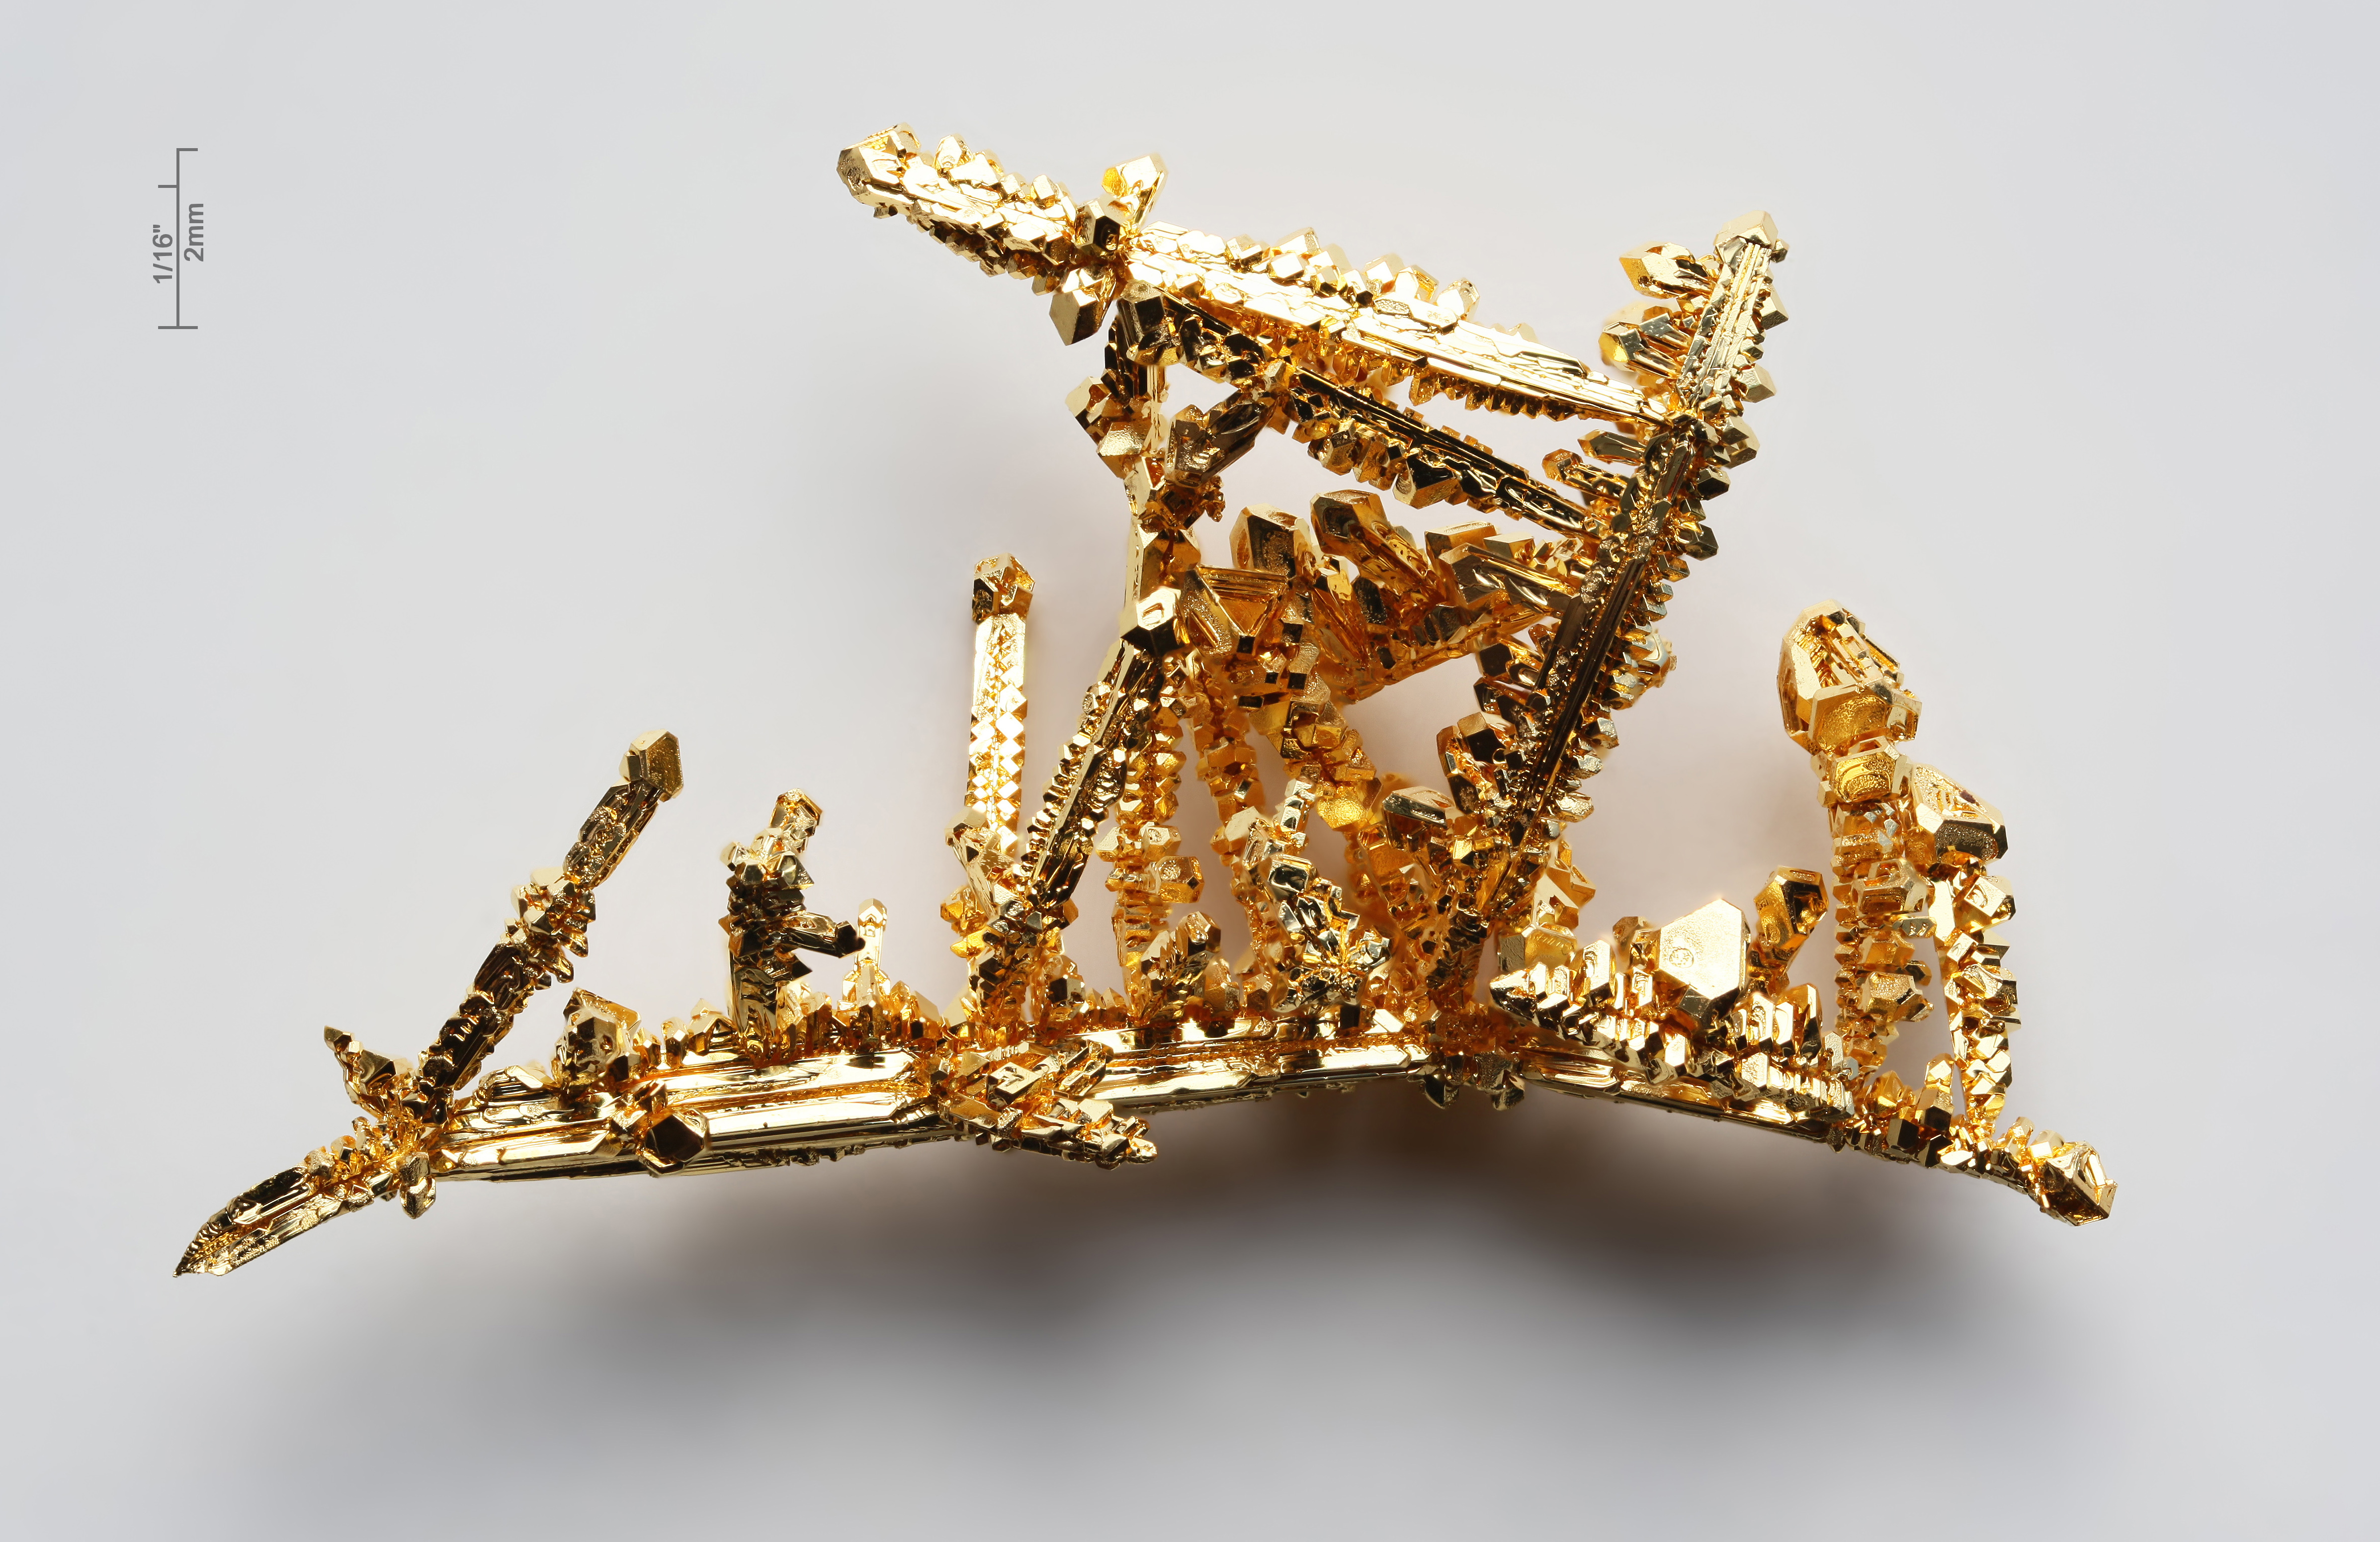
\includegraphics[width=\linewidth,scale=0.5]{chapter8/figure6}
%\caption{Warming an aerosol container will increase the pressure of gas inside}
%\end{marginfigure}%%%%%%%MARGIN FIGURE
\item[\docfilehook{Volume-Temperature change}{Volume-Temperature change}] 
Imagine you cool down a balloon at fixed pressure (under the atmosphere). What would happen to the balloon's volume? Based on Charle's law, its volume will decrease:
\begin{equation*}
\boxed{\frac{V} {T}=c \quad or \quad   \frac{V_1} {T_1}=\frac{V_2} {T_2}} \quad \textcolor{blue}{\text{Charle's law}}
\end{equation*}
where:
\begin{where}
 \item $V_1, T_1$   are the initial volume and temperature
 \item $V_2, T_2$   are the final volume and temperature
   \item $c$   is a constant
\end{where}


%\begin{marginfigure}[0cm]%%%%%%%MARGIN FIGURE
%\includegraphics {chapter8/figure7}
%\caption{An hot air balloon will rise up as air's density decreases with temperature}
%\end{marginfigure}%%%%%%%MARGIN FIGURE

\item[\docfilehook{Volume-Moles change}{Volume-Moles change}] 
Imagine a hot air balloon. Air comes in and out of the balloon as the balloon is not closed balloon. Hence the pressure inside the balloon is just the atmospheric pressure. Also as the balloon is in contact with the air, its temperature will be constant, resulting from the thermal equilibrium between the inside of the balloon and the atmoshphere. If you inflate the balloon with hot air, the volume of the balloon and the number of moles are related by Avogadro's law:
\begin{equation*}
\boxed{ \frac{V} {n}=c \quad or \quad   \frac{V_1} {n_1}=\frac{V_2} {n_2}} \quad \textcolor{blue}{\text{Avogadro's law}}
\end{equation*}
where:
\begin{where}
 \item $V_1, n_1$   are the initial volume and number of moles
 \item $V_2, n_2$   are the final volume and number of moles
   \item $c$   is a constant
\end{where}

\item[\docfilehook{Relating the different variables of a gas}{Relating the different variables of a gas}] 
The questions is now, if we increase the pressure at fixed number of moles and pressure, how do we know if the volume will increase or perhaps decrease? Similarly, if for example the number of gas moles increase at fixed pressure and volume, will the temperature of the gas increase or perhaps decrease. We can answer these questions by means of the ideal gas law. If the variables that we need to relate are in the same side of the equation (e.g. P and V) then if one of the variables increase the other will decrease. Differently, If the gas variables to relate are located in opposite sides of the gas law (e.g. P and T) then both will change in the same direction. For example, let us consider the changes of P and V (at fixed n and T). As they are in the same side of the ideal gas law ($\textcolor{dgreen}{PV}=nRT$), if P increases V will decrease. Differently, for the change of P and T (at fixed V and n), as both variables are in opposite sides of the ideal gas law ($\textcolor{dgreen}PV=nR\textcolor{dgreen}T$), if P increases, T will increase as well.
\end{description}












%\begin{marginfigure}[0cm]%%%%%%%MARGIN FIGURE
%\includegraphics{chapter8/figure5}
%\caption{Each component in a gas mixture exert a partial pressure.}
%\end{marginfigure}%%%%%%%MARGIN FIGURE

\section{Mixtures of gases and gas stoichiometry}
The air is a mixture of different gases. It contains oxygen (\ce{O2}) and nitrogen (\ce{N2}) as well as other gases such as carbon dioxide, argon, or water vapor. Only 21\% of the air is made of oxygen and 78.2\% of nitrogen. The other gases represent 0.8\% of the air. The atmospheric pressure is 1 atm and results from the pressure of all the components of the air. Each gas exerts a partial pressure and all combined exert the total atmospheric pressure. In this section you will learn how to work with mixtures of gases. This section also covers the use of the molar volume to relate moles and volume at standard conditions.

\sloppy 
\begin{description}
\item[\docfilehook{Molar volume}{Molar volume}] 
If we work at STP conditions the volume of one mole of gas equals to 22.4L, and we refer to this relationship as the molar volume.%\resizeableyellownote{2.5}{1}{Add this relation into your flashcard.}
\begin{equation*}
\boxed{  \frac{1 \text{mol}} {22.4\text{ L at STP}} } \quad \textcolor{blue}{\text{Molar Volume}}
\end{equation*}
This relationship allows us to carry stoichiometric calculations in chemical reaction involving gases.


\item[\docfilehook{stoichiometry and gases}{}] If you encounter chemical reactions with gases, the molar volume relation allows you to carry stoichiometric calculations. Why is this important? Imagine you have this reaction:
\begin{center}\ce{ $\underset{\text{\large 3L}}{\ce{2H2(g)}}$ + O2(g)  -> $\underset{\text{\large xL}}{\ce{2H2O(g)}}$  } \end{center}
Gases are measured by means of their pressure and is more convenient to speak about liters of hydrogen than moles of hydrogen or grams of hydrogen, as hydrogen is a gas. This way, if we start by mixing 3L of \ce{H2} we would like to know how much water is being produced. In order to calculate this, we will use the stoichiometric coefficients. In previous chapters we saw that these numbers represent moles and the units of these numbers is mol. If the reaction deals with gases you want to interpret the stoichiometric coefficients in terms of liters. This way:
\begin{equation*}
x=3\cancel{\text{ L of }\ce{H2}} \times \dfrac{\text{2 L of }\ce{H2O}}{2\cancel{\text{ L of \ce{H2}}}}=3\text{ L of }\ce{H2O}.
\end{equation*}
Overall, if we mix three litters of hydrogen we obtain 3L of water.
In case we know the litters of any of the reactants and we need to calculate the moles of product, then we have to add an extra step to transform litters into moles.


\begin{example} %%%%%%%%%%%%%%%%%%%%%%%% EXAMPLE BOX
Hydrogen gas reacts with oxygen gas to produce water vapor according to the following equation:
\begin{center}\ce{  2H2(g)  + $\underset{\text{\large 2L}}{\ce{O2(g)   }}$  -> $\underset{\text{\large x mol}}{\ce{2H2O(g)}}$  } \end{center}
Calculate the number of moles of water produced from 2L of oxygen at STP conditions.
\\
\textlcsc{ \textcolor{dgreen}{\Large \textbf{Solution}} }\\
We will solve the problem in a single line, first relating the liters of oxygen and litters of water produced and finally converting litters of water into moles of water using the molar volume. Remember when there are gases in the reaction, the stoichiometric coefficients can be interpreted in terms of liters:
\begin{equation*}
x=2L\cancel{\text{ L of }\ce{O2}} \times \dfrac{\cancel{\text{2 L of }\ce{H2O}}}{2\cancel{\text{ L of \ce{O2}}}} \times   \dfrac{\text{1 mol of }\ce{H2O}}{22.4 \cancel{\text{L of \ce{H2O}}}}      =0.178\text{ mol of }\ce{H2O}.
\end{equation*}
We have that two liters of oxygen produce four liters of water. At the same time, 22.4L of water--or any other gas--is 1 moles of that gas. So four L of water are 0.17moles of water.
\\
\faDiamond\ \textlcsc{ \textcolor{dgreen}{\Large \textbf{Study Check}} }\\
Hydrogen gas reacts with nitrogen (MW=28 g/mol) gas to produce ammonia at STP conditions according to the following equation:
\begin{center}\ce{  3H2(g)  + $\underset{\text{\large 2L}}{\ce{N2(g)   }}$  -> $\underset{\text{\large x g}}{\ce{2NH3(g)}}$  } \end{center}
Calculate the number of grams of ammonia produced from 0.5L of nitrogen.
\\
\flushright Answer: 5g.
\end{example}%%%%%%%%%%%%%%%%%%%%%%%% EXAMPLE BOX
\item[\docfilehook{Partial and total pressure}{Partial and total pressure}] 
Imagine you have a container with 1atm of Ar, and nother container of the same volume containing 1 atm of Ne. If you combine the containers into a single container (and temperature does not change), hence the pressure in the container will result from both gases and will be 2 atm. Inside the mixed container, 2 atm will the the total pressure ($P_{Total}$), whereas the partial pressure of each gas ($p_{1}$ and $p_{2}$) will be 1 atm. Dalton's Law says that the total pressure results from adding the partial pressure of each gas. For a gas mixture with $n$ components:
\begin{equation*}
\boxed{  P_{Total}=p_1+p_2+\dots p_n} \quad \textcolor{blue}{\text{Dalton's Law}}
\end{equation*}


\begin{example} %%%%%%%%%%%%%%%%%%%%%%%% EXAMPLE BOX
Medical Air is a odorless gas made mostly of nitrogen and oxygen,  administer by ventilator in hospital settings with an operating gauge pressure of 3 atm. If the oxygen pressure inside a container is 2.37 atm, calculate the partial pressure of nitrogen in the mixture. 
\\
\textlcsc{ \textcolor{dgreen}{\Large \textbf{Solution}} }\\
The problem gives the total pressure of the mixture and the partial pressure of one of the components. By using Dalton's law, we know that if the total pressure is 3atm and the partial pressure of oxygen is 2.37, hence the partial pressure of the other component has to be 0.63 atm.
\\
\faDiamond\ \textlcsc{ \textcolor{dgreen}{\Large \textbf{Study Check}} }\\
Entonox is a medicinal mixture of dinitrogen oxide (\ce{N2O}) and oxygen (\ce{O2}). The pressure \ce{N2O} in a entonox container is 2 atm and the oxygen pressure is 1520 mmHg as well. Calculate the total pressure in atm in a Entonox container.
\\
\flushright Answer: 4 atm.
\end{example}%%%%%%%%%%%%%%%%%%%%%%%% EXAMPLE BOX
%%%%%%%%%%%%%%%%%%%%%%
\begin{figure}
\begin{tikzpicture}[thick,scale=0.9, every node/.style={transform shape}]
\begin{scope}
   \filldraw [draw=none,drop shadow={top color=black, bottom color=white, shadow xshift=.3em,  shadow yshift=-.0em,rounded corners }, rounded corners, top color= blue, bottom color=white](0,0) circle [radius=.2cm];
      \filldraw [draw=none,drop shadow={top color=black, bottom color=white, shadow xshift=.3em,  shadow yshift=-.0em,rounded corners }, rounded corners, top color= blue, bottom color=white](1,1) circle [radius=.2cm];
         \filldraw [draw=none,drop shadow={top color=black, bottom color=white, shadow xshift=.3em,  shadow yshift=-.0em,rounded corners }, rounded corners, top color= blue, bottom color=white](-.2,2) circle [radius=.2cm];
   \filldraw [draw=none,drop shadow={top color=black, bottom color=white, shadow xshift=.3em,  shadow yshift=-.0em,rounded corners }, rounded corners, top color= blue, bottom color=white](0,3.5) circle [radius=.2cm];
         \filldraw [draw=none,drop shadow={top color=black, bottom color=white, shadow xshift=.3em,  shadow yshift=-.0em,rounded corners }, rounded corners, top color= blue, bottom color=white](-1,1.2) circle [radius=.2cm];
\flask{0,0}{100}{};
\node[text width=1cm] at (.5,-1)  {\large $p_{A}$};
    
\end{scope}
\begin{scope}[shift={(4,0)}]
   \filldraw [draw=none,drop shadow={top color=black, bottom color=white, shadow xshift=.3em,  shadow yshift=-.0em,rounded corners }, rounded corners, top color= red, bottom color=white](-1,0.3) circle [radius=.2cm];
      \filldraw [draw=none,drop shadow={top color=black, bottom color=white, shadow xshift=.3em,  shadow yshift=-.0em,rounded corners }, rounded corners, top color= red, bottom color=white](0.9,1.5) circle [radius=.2cm];
         \filldraw [draw=none,drop shadow={top color=black, bottom color=white, shadow xshift=.3em,  shadow yshift=-.0em,rounded corners }, rounded corners, top color= red, bottom color=white](.6,0.5) circle [radius=.2cm];
   \filldraw [draw=none,drop shadow={top color=black, bottom color=white, shadow xshift=.3em,  shadow yshift=-.0em,rounded corners }, rounded corners, top color= red, bottom color=white](0.3,3.) circle [radius=.2cm];
         \filldraw [draw=none,drop shadow={top color=black, bottom color=white, shadow xshift=.3em,  shadow yshift=-.0em,rounded corners }, rounded corners, top color= red, bottom color=white](-.8,1.) circle [radius=.2cm];
               \filldraw [draw=none,drop shadow={top color=black, bottom color=white, shadow xshift=.3em,  shadow yshift=-.0em,rounded corners }, rounded corners, top color= red, bottom color=white](-0.1,2.0) circle [radius=.2cm];
\flask{0,0}{300}{};
\node[text width=1cm] at (.5,-1)  {\large $p_{B}$};

\end{scope}
\begin{scope}[shift={(8,0)}]
   \filldraw [draw=none,drop shadow={top color=black, bottom color=white, shadow xshift=.3em,  shadow yshift=-.0em,rounded corners }, rounded corners, top color= red, bottom color=white](-1,0.3) circle [radius=.2cm];
      \filldraw [draw=none,drop shadow={top color=black, bottom color=white, shadow xshift=.3em,  shadow yshift=-.0em,rounded corners }, rounded corners, top color= red, bottom color=white](0.9,1.5) circle [radius=.2cm];
         \filldraw [draw=none,drop shadow={top color=black, bottom color=white, shadow xshift=.3em,  shadow yshift=-.0em,rounded corners }, rounded corners, top color= red, bottom color=white](.6,0.5) circle [radius=.2cm];
   \filldraw [draw=none,drop shadow={top color=black, bottom color=white, shadow xshift=.3em,  shadow yshift=-.0em,rounded corners }, rounded corners, top color= red, bottom color=white](0.3,3.) circle [radius=.2cm];
         \filldraw [draw=none,drop shadow={top color=black, bottom color=white, shadow xshift=.3em,  shadow yshift=-.0em,rounded corners }, rounded corners, top color= red, bottom color=white](-.8,1.) circle [radius=.2cm];
               \filldraw [draw=none,drop shadow={top color=black, bottom color=white, shadow xshift=.3em,  shadow yshift=-.0em,rounded corners }, rounded corners, top color= red, bottom color=white](-0.1,2.0) circle [radius=.2cm];
               
               
\filldraw [draw=none,drop shadow={top color=black, bottom color=white, shadow xshift=.3em,  shadow yshift=-.0em,rounded corners }, rounded corners, top color= blue, bottom color=white](0,0) circle [radius=.2cm];
      \filldraw [draw=none,drop shadow={top color=black, bottom color=white, shadow xshift=.3em,  shadow yshift=-.0em,rounded corners }, rounded corners, top color= blue, bottom color=white](1,1) circle [radius=.2cm];
         \filldraw [draw=none,drop shadow={top color=black, bottom color=white, shadow xshift=.3em,  shadow yshift=-.0em,rounded corners }, rounded corners, top color= blue, bottom color=white](-.9,2) circle [radius=.2cm];
   \filldraw [draw=none,drop shadow={top color=black, bottom color=white, shadow xshift=.3em,  shadow yshift=-.0em,rounded corners }, rounded corners, top color= blue, bottom color=white](0,3.5) circle [radius=.2cm];
         \filldraw [draw=none,drop shadow={top color=black, bottom color=white, shadow xshift=.3em,  shadow yshift=-.0em,rounded corners }, rounded corners, top color= blue, bottom color=white](-0,1.2) circle [radius=.2cm];
\flask{0,0}{400}{};
\node[text width=2cm] at (.5,-1)  {\large $p_{A}+p_{B}$};
\end{scope}
\end{tikzpicture}
\caption{A visual representation of Dalton's law of partial pressure: after adding two different gases with different partial pressured, the final pressure is the result of adding both partial pressures.}
\label{fig:{\chapterlabel}10}
\end{figure}
%%%%%%%%%%%%%%%%%%%%%%

In Figure \ref{fig:{\chapterlabel}10}, we have that after combining two gases with different partial pressures the resulting pressure is the addition of both partial pressured.

\item[\docfilehook{Partial pressure of a gas in a mixture}{ }] For a mixture with different gases, the partial pressure of a given gas ($A$) will depend on the number of moles of that particular gas and the overall volume of the mixture
\begin{equation*}
\boxed{  p_A = \frac{n_A RT }{V }    }
\end{equation*}

\item[\docfilehook{Mole fraction}{Mole fraction}] The mole fraction ($X_A$) of a gas (A) in a mixture of gas is just the number of moles of this gas over the total number of moles in the mixture. The larger the mole fraction of a gas in a mixture the more molecules of that specific gas are there in the mixture with respect to all components. One can express the morel fraction in terms of partial pressures also, as the pressure of a given gas over the total pressure. For a mixture with $n$ components:
\begin{equation*}
\boxed{  X_A = \frac{n_A}{n_A + n_B + \dots + n_n}\;\; \;    or\;\; \;   \frac{p_A}{p_A + p_B + \dots + p_n} }
\end{equation*}
For a mixture of gases, the partial pressure of a gas ($p_A$) is related to the mole fraction of that gas ($X_A$) and the total pressure of the mixture of gases ($P_{Total}$):
\begin{equation*}
\boxed{  p_A=X_A\cdot P_{Total}}
\end{equation*}
\begin{example} %%%%%%%%%%%%%%%%%%%%%%%% EXAMPLE BOX
A mixture of gases with a total pressure of 2 atm contains 3 moles of Ar, 3 moles of He and 1 moles of Ne. Calculate the partial pressure of each component on the mixture. 
\\
\textlcsc{ \textcolor{dgreen}{\Large \textbf{Solution}} }\\
We calculate first the mole fraction for each component of the mixture. As the total number of moles if 7 moles and there are 3 moles of Ar, its mole fraction is 0.43. Similarly, the mole fraction for He is 0.43 and for Ne is 0.14. To calculate the partial pressure of each gas you just need to multiply its mole fraction by the total pressure (2 atm). Hence: $p_{Ar}$=0.86atm, $p_{He}$=0.86atm and $p_{Ne}$=0.28atm
\\
\faDiamond\ \textlcsc{ \textcolor{dgreen}{\Large \textbf{Study Check}} }\\
A mixture of gases with a total pressure of 5 atm contains 1 mol of Ar and 1 mol of He. Calculate the partial pressure of each component on the mixture. 
\\
\flushright Answer: $p_{Ar}$=2.5 atm, $p_{He}$=2.5atm.
\end{example}%%%%%%%%%%%%%%%%%%%%%%%% EXAMPLE BOX

\item[\docfilehook{Collecting gas over water: use of partial pressures}{}] 
\begin{figure}\begin{center}
\begin{tikzpicture} \node (a) at (0,0) {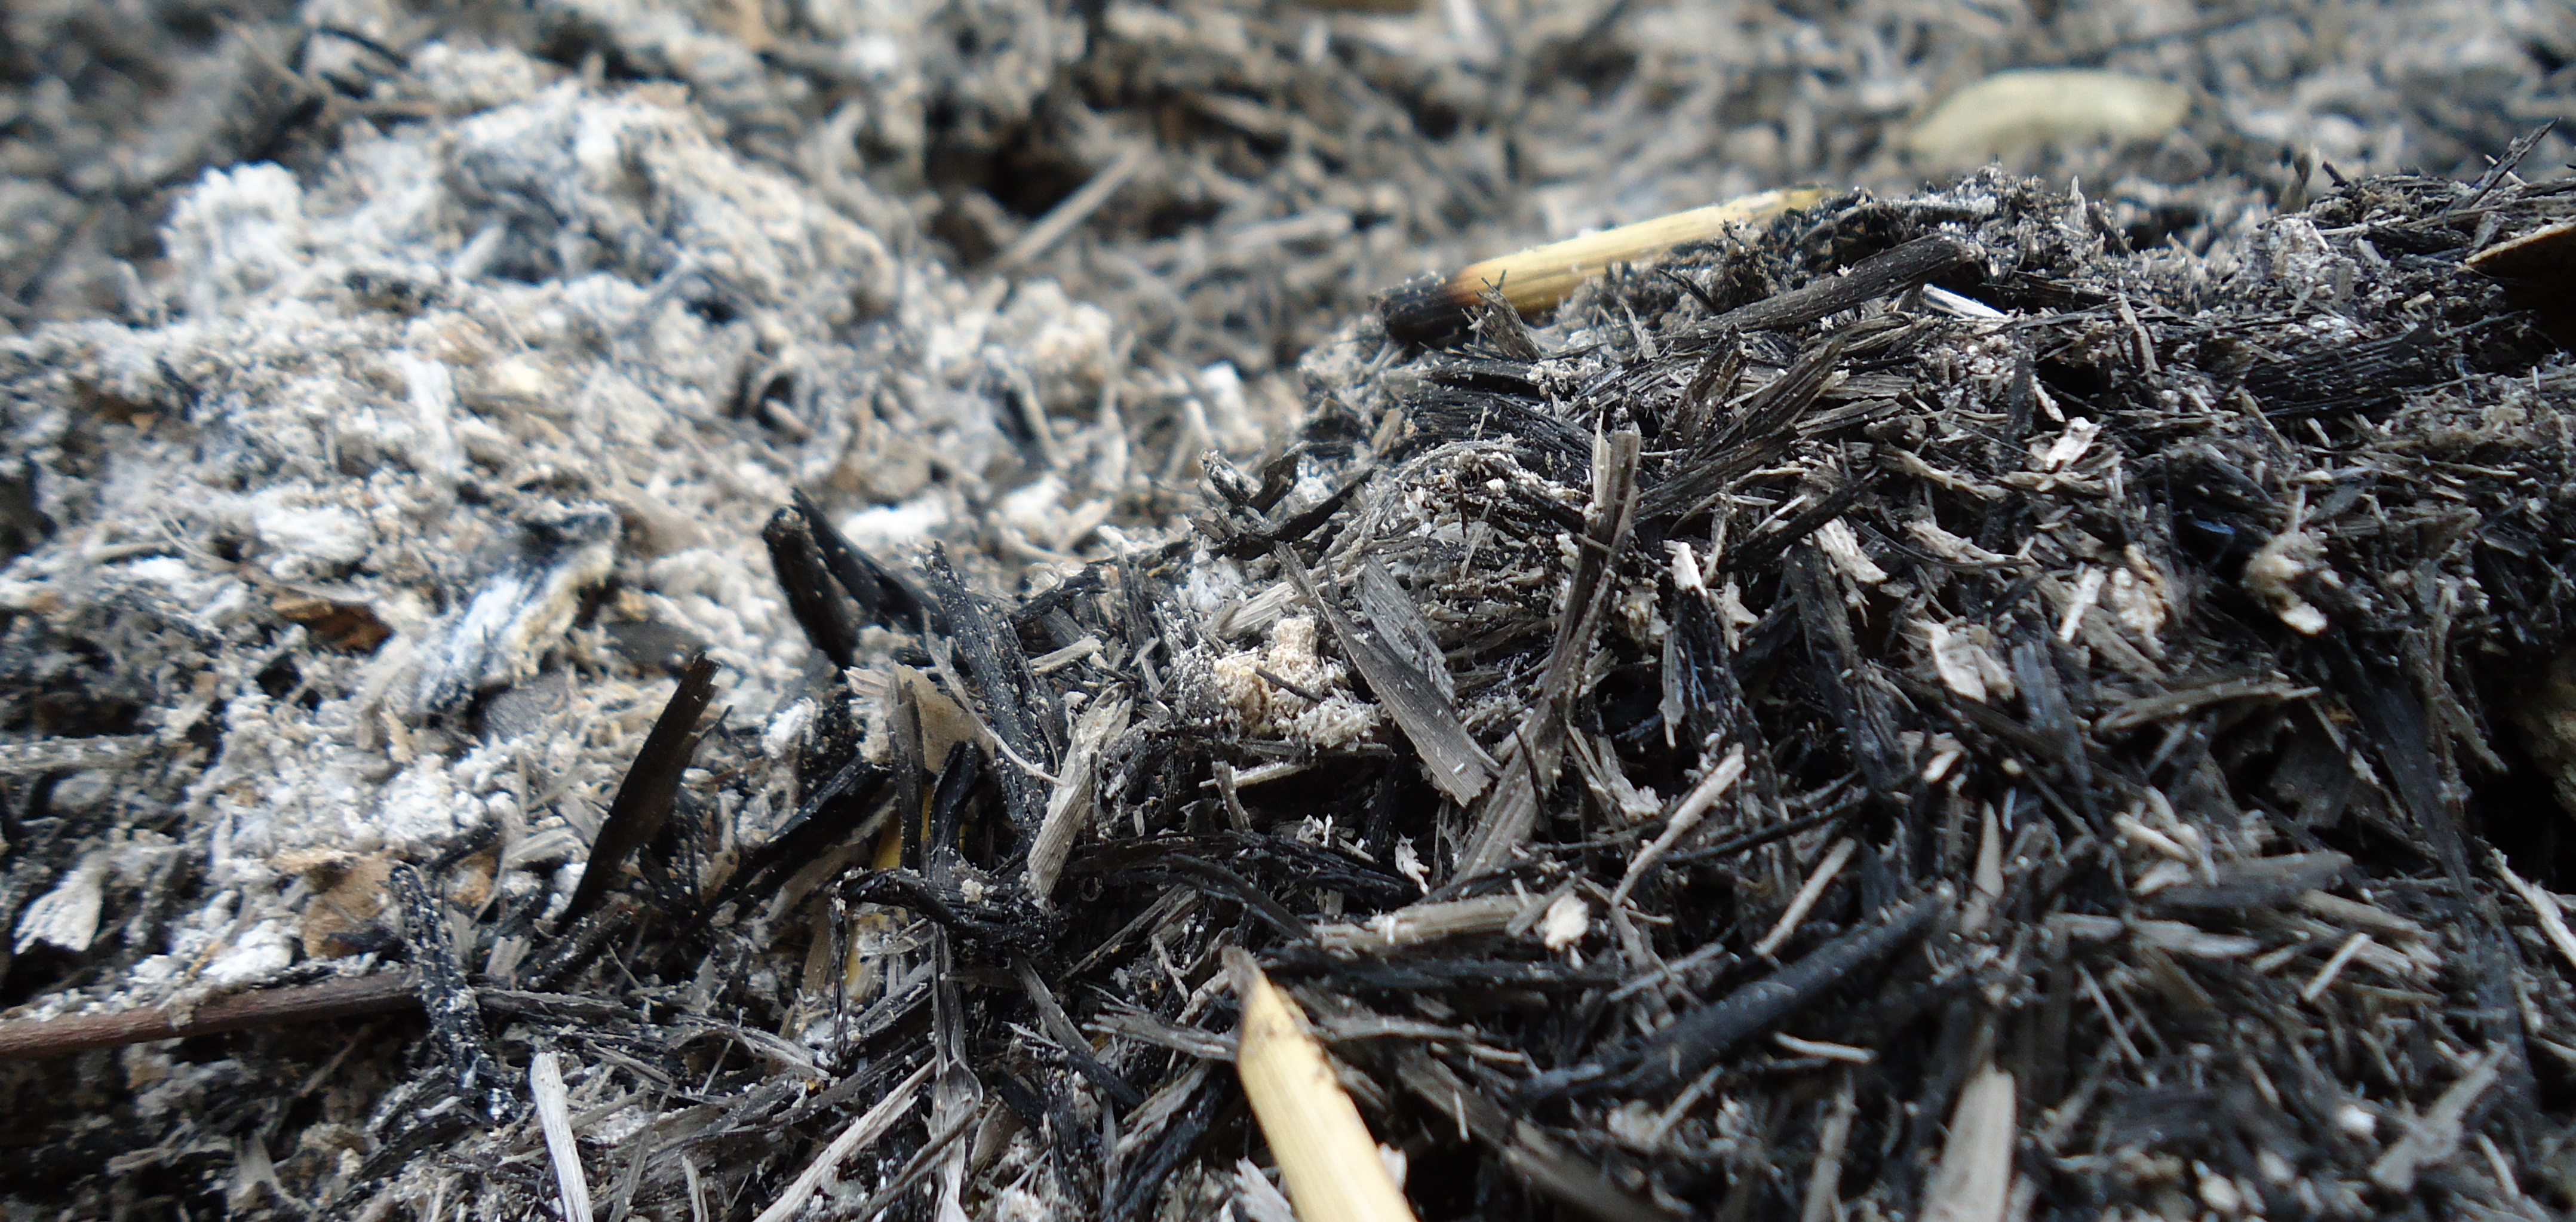
\includegraphics[width=6cm, height=6cm]{chapter8/figure8}} node[rotate=90, font=\tiny] at ([yshift=.5cm,xshift=.1cm]a.south east) {\textsuperscript{\textcopyright} Pst-Labo} ;
\draw[thin] (2.,0.7) -- ++(1,1) node [right,fill=white,font=\small,scale=0.7] {\textcolor{red}{\ce{O2_{(g)}}} +\ce{H2O_{(g)}}};
\draw[thin] (2.,0.1) -- ++(1,-1) node [right,fill=white,font=\small,scale=0.7] {\ce{H2O_{(l)}}};
\draw [->,red] node[font=\small,scale=0.7, xshift=-4.5cm, yshift=.8cm] {\ce{2KClO3_{(s)}}}   (-2.5,0.5) to [out=0,in=360] (-2.5,1.2) node[font=\small,scale=0.7, xshift=-1.5cm, yshift=.0cm] {\ce{2KCl_{(s)} + 3O2_{(g)}}} ; 
\end{tikzpicture}
\label{fig:{\chapterlabel}8}
\caption{Apparatus for measuring the amount of gas produced by a reaction over water.}
\end{center}\end{figure}


Numerous reaction produce gases. As an example, potassium chlorate decomposes to produce oxygen gas:
\begin{center}\ce{2KClO3_{(s)} -> 2KCl_{(s)} + 3O2_{(g)}}\end{center}
The volume of gas produced by a chemical reaction is collected often times over water. Gas bubbles go through water being collected in an apparatus similar to the one represented in Figure \ref{fig:{\chapterlabel}8}. 

As the gas is collected over water, with the gas produced by the reaction, we will also find water molecules that will exhibit a certain partial pressure. In another words, we will collect a mixture of two gases, the gas produced by the reaction and water. The partial pressure of the gas produced will be:
\begin{equation*}
\boxed{  P_{gas}=P_{total}- P_{\ce{H2O}}  }  
 \end{equation*}




The partial pressure of water, also called the vapor pressure of water, depends on temperature and its values can be found in Table \ref{tab:{\chapterlabel}1}. For example, at 25$^{\circ}$C, the vapor pressure of water in the atmosphere is 0.0313 atm and at 100$^{\circ}$C is equal to 1atm. When liquids boil, they vapor pressure is equal to the atmospheric pressure, that is the reason behind the vapor pressure of water being 1 atm at 100$^{\circ}$C, the boiling point of water.



\begin{center}
\refstepcounter{table} \label{tab:{\chapterlabel}1}
%\begin{table}[ht]
\fontfamily{ppl}\selectfont
\begin{tabular}{llllllllll}
\rowcolor{black!45}
\toprule
\multicolumn{10}{l}{\hypersetup{colorlinks,linkcolor={white}} \cellcolor{black}\color{white}\bfseries\small Table \ref{tab:{\chapterlabel}1} Vapor pressure, partial water pressure as a function of temperature } \\
\midrule
 \rowcolor{gray!10} T$^{\circ}$C & P(atm) & T$^{\circ}$C & P(atm) & T$^{\circ}$C &  P(atm) & T$^{\circ}$C &  P(atm)& T$^{\circ}$C &  P(atm)\\
\midrule
  5	 & 	0.0086&	 25	  &	0.0313&	45	  &	0.0946&	65	  &	0.2469&	85	 & 	0.5706	\\
10	  &	0.0121&	30	  &	0.0419&	50	 & 	0.1218&	70	 & 	0.3077&	90	  &	0.6920	\\
15	  &	0.0168&	35	  &	0.0555&	55	  &	0.1555&	75	 & 	0.3806&	95	 & 	0.8342	\\
20	  &	0.0231&	40	  &	0.0728&	60	  &	0.1967&	80	 & 	0.4675&	100	  &	1.0000	\\
 \bottomrule
\end{tabular}\end{center}

\begin{example} %%%%%%%%%%%%%%%%%%%%%%%% EXAMPLE BOX
Oxygen is collected over water in the decomposition of potassium chlorate:
\begin{center}\ce{2KClO3_{(s)} -> 2KCl_{(s)} + 3O2_{(g)}}\end{center}
Given that 20mL of gas are collected at 30$^{\circ}$C at a pressure of 0.9atm, and that the vapor pressure of water at that temperature is 0.0419 atm, calculate the number of moles of oxygen collected.
\\
\textlcsc{ \textcolor{dgreen}{\Large \textbf{Solution}} }\\
In order to calculate the number of moles of oxygen collected we need the partial pressure of oxygen, the temperature and the volume. We have that as the total pressure is 0.9atm and the partial pressure of water is 0.0419 atm, then the partial pressure of oxygen should be $0.9-0.0419$ atm, that is 0.481 atm. As we have the temperature (303K) and the volume (0.02L), we can calculate the number of moles of oxygen:
\[n_{\ce{O2}}=\frac{P_{\ce{O2}}V}{RT}=\frac{0.481\cdot 0.02}{0.082\cdot 303}=3.8\times 10^{-4}\text{moles of }\ce{O2}\]
\\
\faDiamond\ \textlcsc{ \textcolor{dgreen}{\Large \textbf{Study Check}} }\\
Oxygen is collected over water in the decomposition of potassium chlorate:
\begin{center}\ce{2KClO3_{(s)} -> 2KCl_{(s)} + 3O2_{(g)}}\end{center}
Given that 10mL of gas are collected at 35$^{\circ}$C at a pressure of 0.5atm, and that the vapor pressure of water at that temperature is 0.0555 atm, calculate the number of moles of \ce{KClO3} decomposed.
\\
\flushright Answer: $1.2\times 10^{-4}$ moles of \ce{KClO3}.
\end{example}%%%%%%%%%%%%%%%%%%%%%%%% EXAMPLE BOX




\end{description}


\section{Real gases and the kinetic molecular theory of gases }
Until now we have discusses ideal gases. Ideal gases represent very diluted gases in which the gas particles do not see each other, as they are apart. The particles of an ideal gas are very minute without a volume. The collisions between the particles and the walls of the container are elastic--this means the gas molecules do not loose any energy. As you can imagine, no gas is an ideal gas, as this is just an ideal model. This section will cover the properties of real gases, in which the gas particles interact among themselves. We will also discuss the kinetic molecular theory with a particular emphasis on particle average velocity--this is technically called root mean square velocity, $v_{RMS}$. 
\sloppy 
\begin{description}
\item[\docfilehook{Van der Waals equation for real gases}{}] 
When we take into account the fact that the particles of a gas interact with each other the formula of the ideal gases do not work anymore. Instead, we can use the Van der Waals equation for real gases that functions in a very similar way.
\begin{equation*}\begin{split}
\boxed{  P=\frac{nRT}{V-nb}-\frac{n^2a}{V^2}} \quad \textcolor{blue}{\text{Van der Waals equation}}
\end{split}\end{equation*}
where:
\begin{where}
 \item $P$   is the pressure of the gas in atm
\item $V$    is the volume of the gas in L 
 \item $n$   is the number of moles of the gas
\item $T$   is the temperature of the gas in K
\item $R$   is the constant of the gas $0.082\frac{\text{atm}\cdot \text{L}}{\text{mol}\cdot \text{K}}$
\item $a$ and $b$   are the Van der Waals constants in units of $\text{atm}\cdot \text{L}^2\cdot \text{mol}^{-2}$ and $\text{L}\cdot \text{mol}$
\end{where}


\item[\docfilehook{The meaning of the Van der Waals constants}{}] 
There are two an der Waals constants: $a$ and $b$. The Van der Waals constant $a$ represent the degree of interaction between the molecules of a gas. The larger these values the more interactions exists between the gas particles. For example, for \ce{He} we have $a=$ 0.0341$\text{atm}\cdot \text{L}^2/\text{mol}^{2}$, whereas for \ce{H2O} we have $a=$ 5.46 $\text{atm}\cdot \text{L}^2/\text{mol}^{2}$. Comparing the values of $a$ for both gases, we can conclude that the interaction between the particles of \ce{He} are very weak and in contrast, the interactions between the particles of \ce{H2O} are stronger. The Van der Waals constant $b$ is related to the molecular size, however, the relationship is not as straightforward as in the case of the $a$ constant.
\begin{center}
\refstepcounter{table} \label{tab:{\chapterlabel}2}
%\begin{table}[ht]
\fontfamily{ppl}\selectfont
\begin{tabular}{llllll}
\rowcolor{black!45}
\toprule
\multicolumn{6}{l}{\hypersetup{colorlinks,linkcolor={white}} \cellcolor{black}\color{white}\bfseries\small Table \ref{tab:{\chapterlabel}2} Van der Waals constants for several gases } \\
\midrule
 \rowcolor{gray!10} gas   & a ($\text{atm}\cdot \text{L}^2/\text{mol}^{2}$)    &   b ($\text{L}/\text{mol}$)  & gas  &a ($\text{atm}\cdot \text{L}^2/\text{mol}^{2}$) &b ($\text{L}/\text{mol}$)   \\
\midrule
 \ce{NH3}	 & 	\multicolumn{1}{c}{4.225} &	  0.0371	& \ce{Ar}	 & 	\multicolumn{1}{c}{1.355} &	  0.03201  	 	\\
\ce{C6H6   }	 & 	\multicolumn{1}{c}{18.24} &	 	0.1154	& \ce{CO}&	\multicolumn{1}{c}{3.640}	&0.04267  	 	\\
\ce{CH4}	 & 	\multicolumn{1}{c}{2.283} &	  0.0427	& \ce{CH3OH}	 & 	\multicolumn{1}{c}{9.649} &	  0.06702 	 	\\
\ce{CS2}&	\multicolumn{1}{c}{11.77}	&0.0768&\ce{Cl2}&	\multicolumn{1}{c}{	6.579}	&0.05622\\
\ce{Ne}&	\multicolumn{1}{c}{	0.2135}	&0.01709&\ce{NO}&	\multicolumn{1}{c}{	1.358}	&0.02789\\
\ce{N2}&	\multicolumn{1}{c}{	1.370}	&0.0387&\ce{NO2}&	\multicolumn{1}{c}{	5.354}	&0.04424\\
 \bottomrule
\end{tabular}\end{center}
		




\begin{example} %%%%%%%%%%%%%%%%%%%%%%%% EXAMPLE BOX
Calculate the pressure of 0.2 moles of water vapor at 500K occupying a volume of 0.1L, using: (a) the ideal gas formula and (b) the Van der Waals formula $a=$ 5.46$\text{atm}\cdot \text{L}^2/\text{mol}^{2}$ and $b=$ 0.0305$\text{L}/\text{mol}$.\\
\textlcsc{ \textcolor{dgreen}{\Large \textbf{Solution}} }\\
We will use the ideal gas formula first, given the number of moles ($n$=0.2 mol), temperature ($T$=500K), pressure ($p$=6 atm) and the volume ($V$=0.1L).
\begin{equation*}
P=\frac{nRT}{V}=\frac{0.2\times 0.083\times 500}{0.1}=82atm   
\end{equation*}
Now, using the Van der Waals formula:
\begin{equation*}\begin{split}
P=\frac{nRT}{V-nb}-\frac{n^2a}{V^2}= \frac{0.2\times 0.083\times 500}{0.1-0.2\times 0.0305}-\frac{0.2^2\times 5.46}{0.1^2}=65atm 
\end{split}\end{equation*}
Both values are very different and this is consistent with the fact that water vapor does not behave as an ideal gas.
\\
\faDiamond\ \textlcsc{ \textcolor{dgreen}{\Large \textbf{Study Check}} }\\
Calculate the pressure of 0.9 moles of ammonia gas at 900K occupying a volume of 0.1L, using: (a) the ideal gas formula and (b) the Van der Waals formula $a=$ 4.17$\text{atm}\cdot \text{L}^2/\text{mol}^{2}$ and $b=$ 0.0371$\text{L}/\text{mol}$.\\
\flushright Answer: 664 atm;659 atm.
\end{example}%%%%%%%%%%%%%%%%%%%%%%%% EXAMPLE BOX
\item[\docfilehook{Kinetic theory of gases}{Kinetic theory of gases}] 
%\begin{marginfigure}[0cm]%%%%%%%MARGIN FIGURE
%\includegraphics{chapter8/figure3}
%\caption{The particles of a gas move fast.}
%\end{marginfigure}%%%%%%%MARGIN FIGURE
The kinetic theory of gases is a model that explain the properties of gases. This theory envisions a gas in the form of a set of moving particles. Some of the ideas behind this model are: 
\begin{itemize}
\item  The particles of a gas are in constant motion and move very fast.
\item On its movement, gas particles collide with each other changing paths, and collide with the walls of its container exerting pressure.
\item  Gas particles are far apart from each other, barely interacting.
\item The average kinetic energy of the particles of a gas (this is the energy of the particles due to movement) is proportional to the temperature of the gas.
\end{itemize}
By means of the kinetic theory we can rationalize the different properties of a gas. As the particles of a gas are in constant motion and apart from each other they fill and occupy the same volume of its container. The temperature of a gas is related to its kinetic energy, that is, the average speed of the gas particles. Also, as the gas particles collide with the container's wall, they exert pressure. The kinetic theory of gases explain for example how room fresheners work. As you spray the room, the molecules of the perfume in a gas state move fast and occupy the room.
The kinetic molecular theory of the gases gives a molecular-based description of the temperature of a gas--among other properties. The ideal gas law is an experimental law; this means is a law that comes from measuring and carrying experiments. However, this law does not provide any reasons behind the behavior of gases, ideal or real. The kinetic molecular theory provides a molecular description of temperature. In particular one of the outcomes of this theory is that the average velocity of a gas particle depends on the square root of the temperature of the gas. More precisely, the way this theory describe velocity is in the form of a \emph{root mean square velocity} $v_{RMS}$, that is, as an average of the velocity of each particle. The formula that connects the the root mean square velocity with temperature is:

\begin{equation*}\begin{split}
\boxed{  v_{RMS}=\sqrt{   \frac{3000RT}{MW} }   } \quad \textcolor{blue}{\text{root mean square velocity formula}}
\end{split}\end{equation*}
where:
\begin{where}
 \item $MW$   is the molecular weight of the gas in g/mol
\item $T$   is the temperature of the gas in K
\item $R$   is the constant of the gas in energy units 8.314 $J\cdot K^{-1}\cdot \text{mol}^{-1} $
\item $v_{RMS}$ is the root mean square velocity in $m/s$
\end{where}
It is important to notice that the root mean square velocity depends on temperature--the more temperature the more velocity-- and is inverssely proportional to the molecular weight of the gas--the heavier the mass the lower velocity.


\begin{example} %%%%%%%%%%%%%%%%%%%%%%%% EXAMPLE BOX
Order the following molecules in increasing order of root mean square velocity: \ce{Ne}, \ce{CO2} and \ce{H2O}.\\
\textlcsc{ \textcolor{dgreen}{\Large \textbf{Solution}} }\\
Root mean square velocity is inversely proportional to the molecular weight of the gas; hence, the larger the mass the lower velocity. If we compare the molecular weight of the gases: \ce{Ne}(MW=20g/mol), \ce{CO2}(MW=44g/mol) and \ce{H2O}(MW=18g/mol). The root mean square velocity of water is the largest and the root mean square velocity of carbon dioxide is the smallest.
\\
\faDiamond\ \textlcsc{ \textcolor{dgreen}{\Large \textbf{Study Check}} }\\
Calculate the root mean square velocity of the molecules of water at 25C$^{\circ}$.\\
\flushright Answer: 625m/s.
\end{example}%%%%%%%%%%%%%%%%%%%%%%%% EXAMPLE BOX





\begin{figure*}
\begin{center}
\begin{tikzpicture}[thick,scale=0.8, every node/.style={transform shape}]
\begin{scope}[xshift = -8cm]
\pgfkeys{/pgfplots/linelabel/.style args={#1:#2:#3}{name path global=labelpath,execute at end plot={
\path [name path global = labelpositionline]
(rel axis cs:#1,0) --
(rel axis cs:#1,1);
\draw [help lines,text=black,inner sep=0pt,name intersections={of=labelpath and labelpositionline}] (intersection-1) -- +(#2) node [label={#3}] {};},
}}
\pgfplotsset{ compat  = 1.13,samples = 100,}
\def\kB{1.3806488e-23}% boltzmann constant
\def\temperature{100}% room temperature
\def\Beta{1/(\kB*\temperature)}
\def\amu{1.660538921e-27}% atomar mass unit in kg
\def\mass{28*\amu}
\def\mB{\mass*\Beta}
\begin{axis}[
  axis lines = left,
  domain     = 0:1500,
  xlabel     = Molecular velocity (m/s),
  ylabel     = Number of molecules,
%  xtick      = \empty,
%xmax = 1500,
  ytick      = \empty,
  clip       = false,
]
  \addplot[black, linelabel=0.2:{.6cm,.6cm}: {[black]right:\ce{N2} at $100$K}]		 {sqrt(2/pi)*(\mB)^(3/2)*x^2*exp(-.5*\mB*x^2)};
  \def\temperature{500}% room temperature
\def\Beta{1/(\kB*\temperature)}
\def\amu{1.660538921e-27}% atomar mass unit in kg
\def\mass{28*\amu}
\def\mB{\mass*\Beta}
   \addplot[red, linelabel=0.4:{.6cm,.6cm}: {[red]right:\ce{N2} at $500$K}]{sqrt(2/pi)*(\mB)^(3/2)*x^2*exp(-.5*\mB*x^2)};
  \def\temperature{900}% room temperature
\def\Beta{1/(\kB*\temperature)}
\def\amu{1.660538921e-27}% atomar mass unit in kg
\def\mass{28*\amu}
\def\mB{\mass*\Beta}
  \addplot[blue, linelabel=0.6:{.6cm,.6cm}: {[blue]right:\ce{N2} at $900$K}]{sqrt(2/pi)*(\mB)^(3/2)*x^2*exp(-.5*\mB*x^2)};
\end{axis}
\end{scope}
\begin{scope}[xshift = 3cm]
\pgfkeys{/pgfplots/linelabel/.style args={#1:#2:#3}{name path global=labelpath,execute at end plot={
\path [name path global = labelpositionline]
(rel axis cs:#1,0) --
(rel axis cs:#1,1);
\draw [help lines,text=black,inner sep=0pt,name intersections={of=labelpath and labelpositionline}] (intersection-1) -- +(#2) node [label={#3}] {};},
}}
\pgfplotsset{ compat  = 1.13,samples = 100,}
\def\kB{1.3806488e-23}% boltzmann constant
\def\temperature{300}% room temperature
\def\Beta{1/(\kB*\temperature)}
\def\amu{1.660538921e-27}% atomar mass unit in kg
\def\mass{28*\amu}
\def\mB{\mass*\Beta}
\begin{axis}[
  axis lines = left,
  domain     = 0:1500,
  xlabel     = Molecular velocity (m/s),
  ylabel     = Number of molecules,
%  xtick      = \empty,
%xmax = 1500,
  ytick      = \empty,
  clip       = false,
]
  \addplot[black, linelabel=0.3:{.6cm,.6cm}: {[black]right:\ce{N2} (MW=28amu) at $300$K}]		 {sqrt(2/pi)*(\mB)^(3/2)*x^2*exp(-.5*\mB*x^2)};
  \def\temperature{300}% room temperature
\def\Beta{1/(\kB*\temperature)}
\def\amu{1.660538921e-27}% atomar mass unit in kg
\def\mass{70*\amu}
\def\mB{\mass*\Beta}
   \addplot[red, linelabel=0.2:{.6cm,.6cm}: {[red]right:\ce{Cl2} (MW=71amu) at $300$K}]{sqrt(2/pi)*(\mB)^(3/2)*x^2*exp(-.5*\mB*x^2)};
  \def\temperature{300}% room temperature
\def\Beta{1/(\kB*\temperature)}
\def\amu{1.660538921e-27}% atomar mass unit in kg
\def\mass{253*\amu}
\def\mB{\mass*\Beta}
  \addplot[blue, linelabel=0.1:{.6cm,.6cm}: {[blue]right:\ce{I2} (MW=254amu) at $300$K}]{sqrt(2/pi)*(\mB)^(3/2)*x^2*exp(-.5*\mB*x^2)};
\end{axis}
\end{scope} 
\end{tikzpicture}
\end{center}
\caption{Effect of temperature and mass on the distribution of molecular speeds}
\label{fig:{\chapterlabel}9}
\end{figure*}
\item[\docfilehook{Distribution of velocities}{}] 
The root mean square velocity $v_{RMS}$ is just an average of the square velocities of the gas particles. Still, some particles will have faster velocity than $v_{RMS}$ and other will have slower velocity. The molecular velocities of the particles of a gas follow a distribution which is mass and temperature dependent. 
As shown in Figure \ref{fig:{\chapterlabel}9}, the higher temperature the larger the root square velocity, with a wider distribution of velocities. At the same time, the larger the molar mass of the gas, the smaller the root square velocity with a thiner distribution of velocities.



\end{description}

\clearpage\thispagestyle{empty}\mbox{}\clearpage
\end{document}
